\documentclass[10pt,a4paper]{article}
\usepackage[utf8]{inputenc}
\usepackage[spanish]{babel}
\usepackage{amsmath}
\usepackage{amsfonts}
\usepackage{amssymb}
\usepackage{graphicx}
\usepackage[left=2cm,right=2cm,top=2cm,bottom=2cm]{geometry}
\usepackage[hidelinks]{hyperref}
\usepackage{listings}
% Automatas
\usepackage{tikz}
\usetikzlibrary{automata, positioning, arrows}

\tikzset{
    ->, % makes the edges directed
    >=stealth', % makes the arrow heads bold
    node distance=5cm, % specifies the minimum distance between two nodes. Change if necessary.
    every state/.style={thick, fill=gray!10}, % sets the properties for each ’state’ node
    initial text=$ $ % sets the text that appears on the start arrow
}


\lstset{ frame = single, breaklines = true}

\begin{document}

\begin{titlepage}
\title{\textbf{
	{\Huge  Práctica 4: JADE }\\
	{\Large Sistemas de Ayuda a la Toma de Decisiones }
}}
\author{
	Pedro Allué Tamargo (758267)
	\and
	Juan José Tambo Tambo (755742)
	\and
	Jesús Villacampa Sagaste (755739)
}
\date{\today}
\clearpage\maketitle
\thispagestyle{empty}
\end{titlepage}

\tableofcontents

\newpage
\section{Ejercicio 1}

Para este ejercicio se ha procedido a crear el agente \texttt{Ej1\_Agente}. Este agente deberá saludar al ser creado, por ello se sobrescribirá el método \texttt{setup()}.\\
Para pasar un argumento al agente se hará en la creación del mismo en la opción \emph{arguments} (Figura \ref{fig:creacionAgente}). En el código del agente se utilizarán la siguiente línea:

\begin{lstlisting}
	contador = Integer.parseInt(getArguments()[0].toString());
\end{lstlisting}

Esta línea utilizará el método \texttt{getArguments()} para obtener un array de objetos con los argumentos. Una vez obtenido el primer elemento se convertirá a \texttt{String} y se utilizará el método \texttt{parseInt()} de la clase \emph{wrapper} \texttt{Integer}.\\
Se pide que el agente implemente un comportamiento tipo \texttt{CyclicBehaviour} para decrementar esta variable \texttt{contador} y cuando llegue a 0 termine la ejecución del agente. El comportamiento \texttt{CyclicBehaviour} tiene la peculiaridad de que su método \texttt{done()} siempre devuelve \texttt{false} y por lo tanto no terminará nunca a no ser que se especifique en el método \texttt{action()}. Por lo tanto el código de dicha clase será el siguiente:

\lstinputlisting[label={list:contadorExterno}, language=java]{listings/ContadorExternoBehaviour.java}

El código del agente descrito se puede encontrar en el Listing \ref{list:ej1Agente}.


\newpage
\section{Ejercicio 2}

\subsection{Parte 1}

La comunicación entre los dos agentes (\emph{Ej2\_{}Envia} y \emph{Ej2\_{}Recibe}). 
En el código del comportamiento de \emph{Ej2\_{}Envia} se puede observar como el agente pide datos por entrada estándar para conocer al destinatario del mensaje y el texto a enviar. Tras esto se puede observar que el agente crea un objeto de la clase \texttt{ACLMessage} (\emph{Agent Comunication Language Message}) de tipo \texttt{REQUEST} (petición). Tras esto, crea un objeto que identifica al agente destinatario (\texttt{AID}) y le pasa como parámetros el nombre del agente y además el \emph{booleano} \texttt{AID.ISLOCALNAME} que indica que el nombre del agente solo es válido localmente. Despues se le asigna este identificador \texttt{AID} al destinatario y el texto como contenido del mensaje para después enviarlo utilizando el método \texttt{send()} del agente asociado al comportamiento.\\

En el código del comportamiento del \emph{Ej2\_{}Recibe} ocurre la operación de recepción del mensaje enviado por el agente del comportamiento anterior. En este método \texttt{action} se puede observar como se produce una recepción de un mensaje (\texttt{ACLMessage}) con carácter síncrono, es decir, bloqueante. Tras esto el comportamiento muestra por la salida estándar el nombre del agente del que recibe el mensaje y su contenido.\\

\subsection{Parte 2}

Ahora se pide modificar el código de los comportamientos para que los agentes se reenvíen entre sí el mensaje inicial un número determinado de veces, el cual se pasará como parámetro a uno de los agentes en su creación.\\
Para la implementación de estos comportamientos se ha partido desde una aproximación anterior al apartado anterior. Uno de los agentes será el que envíe primero el mensaje del texto y el otro el que responda con el. Esto ocurrirá tantas veces como se indique en el parámetro.\\

Para la implementación de este comportamiento se han utilizado máquinas de estado finitas (\emph{FSM}). Para el comportamiento que envía el texto por primera vez se ha utilizado el siguiente autómata (Figura \ref{fig:FSMEnvio})

Para el comportamiento del agente de recepción se ha utilizado la máquina de estados complementaria a la de la Figura \ref{fig:FSMEnvio}. Se puede observar la máquina de estados de recepción en la Figura \ref{fig:FSMRecepcion}.

Para la implementación de la máquina de estados en los comportamientos se ha heredado del comportamiento \texttt{FSMBehaviour}. El código del comportamiento de envío se puede encontrar en el Listing \ref{list:FSMEnvioJava} y el código del comportamiento de la recepción en el Listing \ref{list:FSMRecibeJava}.


\section{Ejercicio 3}

En este ejercicio, hay dos agentes, \emph{Ej3\_EmisorPasajeVuelo} y \emph{Ej3\_ReceptorPasajeVuelo}. El funcionamiento consiste en que el primero envía toda la información necesaria para la reserva de un vuelo al segundo.\\

Para la implementación de este comportamiento, en el agente \emph{Ej3\_EmisorPasajeVuelo} se puede observar como el agente pide datos por entrada estándar para conocer al destinatario del mensaje y la información necesaria para reservar el vuelo, que consta del origen, destino, tarifa y aerolínea (Figura \ref{fig:ej3_sender}) y que se encapsula en un objeto de tipo \emph{Ej3\_PasajeVuelo}. Tras esto se puede observar que el agente crea un objeto de la clase \texttt{ACLMessage} (\emph{Agent Comunication Language Message}) de tipo \texttt{CONFIRM} (confirmación). A continuación, crea un objeto que identifica al agente destinatario (\texttt{AID}) y le pasa como parámetros el nombre del agente y además el \emph{booleano} \texttt{AID.ISLOCALNAME} que indica que el nombre del agente solo es válido localmente. Despues se le asigna este identificador \texttt{AID} al destinatario y el objeto \emph{Ej3\_pasajeVuelo} como contenido del mensaje para después enviarlo utilizando el método \texttt{send()} del agente asociado al comportamiento.\\

En el código del comportamiento del \emph{Ej3\_ReceptorPasajeVuelo} ocurre la operación de recepción del mensaje enviado por el agente del comportamiento anterior. En este método \texttt{action} se puede observar como se produce una recepción de un mensaje (\texttt{ACLMessage}) con carácter síncrono, es decir, bloqueante. Tras esto, se comprueba que el mensaje es del tipo \texttt{CONFIRM} y su contenido es un objeto de tipo \emph{Ej3\_PasajeVuelo}. Si se cumplen estas dos condiciones se muestra por la salida estándar toda la información de la reserva del vuelo, que se encuentra encapsulada en el objeto recibido (Figura \ref{fig:ej3_reveiver}). 

\newpage
\section{Anexo 1: Figuras}

% Menu de JADE
\begin{figure}[h!]
\centering
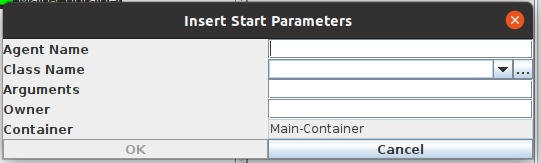
\includegraphics[scale=0.5]{images/arguments.jpeg}
\caption{Captura de pantalla del menú de creación de agentes en \emph{JADE}}
\label{fig:creacionAgente}
\end{figure}

% Automata de envio
\begin{figure}[h!]
\centering
	\begin{tikzpicture}
		% Estados
		\node[state, left](CD) {$Conseguir Datos$};
		\node[state, right of=CD](EN) {$Enviar Numero$};
		\node[state, right of=EN](ET) {$Enviar Texto$};
		\node[state, xshift=3cm, yshift=-6cm](RT) {$Recibir Texto$};
		\node[state, xshift=13cm, yshift=-3cm](F) {$Fin$};
		
		% Transiciones
		\draw (CD) edge node{} (EN);
		\draw (EN) edge node{} (ET);
		\draw (ET) edge[sloped, anchor=center, above, bend left] node{-/contador--} (RT);
		\draw (RT) edge[sloped, anchor=center, above, bend left] node{contador$>$0/-} (ET);
		\draw (RT) edge[sloped, anchor=center, above, bend right] node{contador=0/-} (F);
	\end{tikzpicture}
\caption{Máquina de estados finita del autómata de envío}
\label{fig:FSMEnvio}
\end{figure}

% Automata de recepción
\begin{figure}[h!]
\centering
	\begin{tikzpicture}
		% Estados
		\node[state, left](RN) {$Recibir Numero$};
		\node[state, right of=RN, xshift=7cm](RT) {$Recibir Texto$};
		\node[state, xshift=3cm, yshift=-6cm](ET) {$Enviar Texto$};
		\node[state, xshift=13cm, yshift=-3cm](F) {$Fin$};
		
		% Transiciones
		\draw (RN) edge[sloped, anchor=center, above] node{-/contador=msg.contador, receiver=msg.sender} (RT);
		\draw (RT) edge[sloped, anchor=center, above, bend left] node{-/-} (ET);
		\draw (ET) edge[sloped, anchor=center, above, bend left] node{contador$>$0/-} (RT);
		\draw (ET) edge[sloped, anchor=center, above, bend right] node{contador=0/-} (F);
	\end{tikzpicture}
\caption{Máquina de estados finita del autómata de recepción}
\label{fig:FSMRecepcion}
\end{figure}

% Datos que introduce el Sender en ej3
\begin{figure}[h!]
\centering
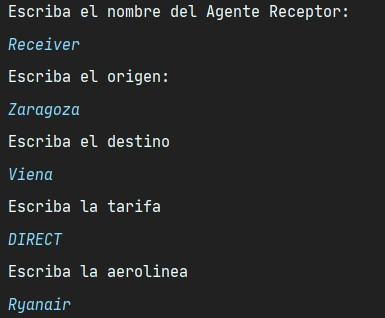
\includegraphics[scale=1]{images/sender_ej3.jpg}
\caption{Captura de pantalla de la información a introducir por entrada estándar para el agente \emph{Ej3\_EmisorPasajeVuelo}}
\label{fig:ej3_sender}
\end{figure}

% Datos que recibe el Receiver en ej3
\begin{figure}[h!]
\centering
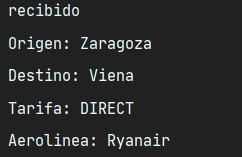
\includegraphics[scale=1]{images/receiver_ej3.jpg}
\caption{Captura de pantalla de la información que recibe\emph{Ej3\_ReceptorPasajeVuelo}}
\label{fig:ej3_reveiver}
\end{figure}

\newpage
\section{Anexo 2: Códigos}

\subsection{Código del agente del Ejercicio 1}

\lstinputlisting[label={list:ej1Agente}, language=java]{listings/ej1Agente.java}

\subsection{Código del comportamiento de la máquina de estados de envío}

\lstinputlisting[label={list:FSMEnvioJava}, language=java]{listings/Ej2_Envia_FSM.java}

\subsection{Código del comportamiento de la máquina de estados de recepción}

\lstinputlisting[label={list:FSMRecibeJava}, language=java]{listings/Ej2_Recibe_FSM.java}

\end{document}